\documentclass[tikz,border=15pt]{standalone}
\usepackage{tikz}
\usepackage{amsmath}
\usepackage{amssymb}
\usetikzlibrary{arrows.meta,positioning,fit,calc,backgrounds,shapes.geometric}

\begin{document}
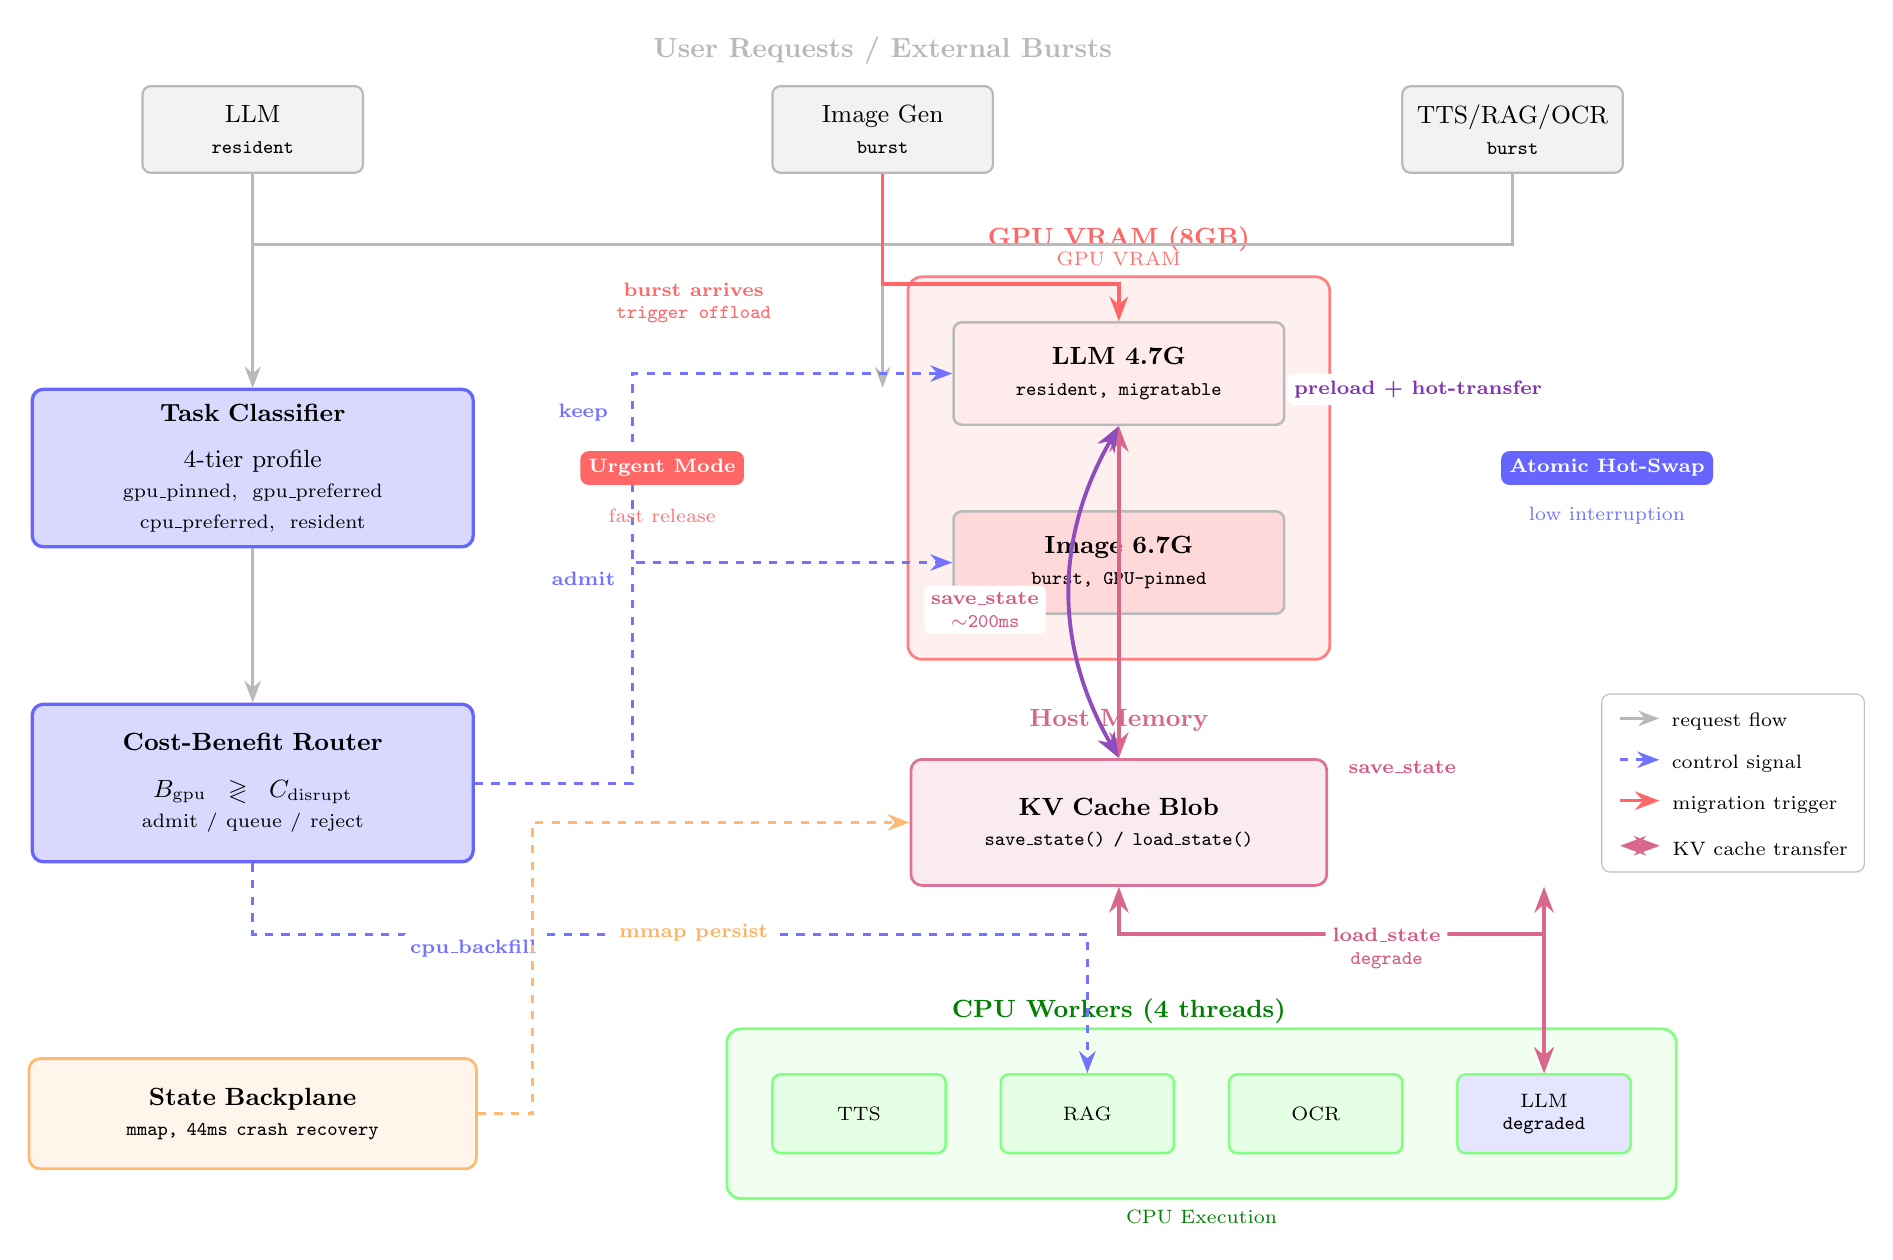
\begin{tikzpicture}[
    font=\small,
    >=Stealth,
    scale=1.0,
    % 节点样式 —— 整体放大、颜色更鲜明
    reqbox/.style={
        draw, rounded corners=3pt, fill=gray!10, draw=gray!55,
        line width=0.8pt, minimum height=11mm, minimum width=28mm,
        align=center, font=\small, inner sep=3pt
    },
    corebox/.style={
        draw, rounded corners=4pt, fill=blue!15, draw=blue!60,
        line width=1.2pt, minimum height=20mm, minimum width=56mm,
        align=center, inner sep=5pt, font=\small
    },
    gpupool/.style={
        draw, rounded corners=5pt, fill=red!6, draw=red!50,
        line width=1.0pt, inner sep=16pt
    },
    cpupool/.style={
        draw, rounded corners=5pt, fill=green!6, draw=green!50,
        line width=1.0pt, inner sep=16pt
    },
    hostbox/.style={
        draw, rounded corners=4pt, fill=purple!8, draw=purple!55,
        line width=1.0pt, minimum width=50mm, minimum height=16mm,
        align=center, inner sep=4pt, font=\small
    },
    slotbox/.style={
        draw, rounded corners=3pt, fill=white, draw=gray!55,
        line width=0.9pt, minimum height=13mm, minimum width=42mm,
        align=center, font=\small, inner sep=3pt
    },
    cpuworker/.style={
        draw, rounded corners=3pt, fill=green!10, draw=green!50,
        line width=0.9pt, minimum height=10mm, minimum width=22mm,
        align=center, font=\scriptsize, inner sep=3pt
    },
    persistbox/.style={
        draw, rounded corners=4pt, fill=orange!8, draw=orange!55,
        line width=1.0pt, minimum width=52mm, minimum height=14mm,
        align=center, font=\small, inner sep=4pt
    },
    modelabel/.style={
        font=\scriptsize\bfseries, text=white, fill=red!60,
        rounded corners=3pt, inner sep=3pt
    },
    uplabel/.style={
        font=\scriptsize\bfseries, text=white, fill=blue!60,
        rounded corners=3pt, inner sep=3pt
    },
    % 箭头样式 —— 加粗、颜色更饱和
    reqarrow/.style={->, >=Stealth, line width=1.0pt, draw=gray!55},
    ctrlarrow/.style={->, >=Stealth, line width=1.1pt, draw=blue!55, dashed},
    triggerarrow/.style={->, >=Stealth, line width=1.3pt, draw=red!60},
    resourcearrow/.style={<->, >=Stealth, line width=1.4pt, draw=purple!60},
    % 标注样式 —— 白底避免被线压住
    flowlabel/.style={
        font=\scriptsize, fill=white, inner sep=2.5pt,
        align=center, rounded corners=2pt
    },
]

% ==================== 顶部：用户请求入口 ====================
\node[font=\normalsize\bfseries, text=gray!55] at (0, 1.8) {User Requests / External Bursts};

\node[reqbox] (req-llm) at (-8.0, 0.8) {LLM\\\texttt{\scriptsize resident}};
\node[reqbox] (req-img) at (0, 0.8) {Image Gen\\\texttt{\scriptsize burst}};
\node[reqbox] (req-aux) at (8.0, 0.8) {TTS/RAG/OCR\\\texttt{\scriptsize burst}};

% ==================== 左侧：控制平面 ====================
\node[corebox, text width=52mm] (classifier) at (-8.0, -3.5) {
    \textbf{Task Classifier}\\[2mm]
    {\small 4-tier profile}\\
    {\scriptsize gpu\_pinned,\; gpu\_preferred}\\
    {\scriptsize cpu\_preferred,\; resident}
};

\node[corebox, text width=52mm] (router) at (-8.0, -7.5) {
    \textbf{Cost-Benefit Router}\\[2mm]
    {\small $B_{\text{gpu}} \gtrless C_{\text{disrupt}}$}\\
    {\scriptsize admit / queue / reject}
};

% ==================== 右侧：资源平面 ====================
% GPU VRAM 池
\node[font=\small\bfseries, text=red!60] at (3.0, -0.6) {GPU VRAM (8GB)};
\node[slotbox, fill=red!8] (gpu-llm) at (3.0, -2.3) {\textbf{LLM 4.7G}\\\texttt{\scriptsize resident, migratable}};
\node[slotbox, fill=red!15] (gpu-img) at (3.0, -4.7) {\textbf{Image 6.7G}\\\texttt{\scriptsize burst, GPU-pinned}};

% Host Memory (KV Cache 存储)
\node[font=\small\bfseries, text=purple!60] at (3.0, -6.7) {Host Memory};
\node[hostbox, text width=50mm] (hostmem) at (3.0, -8.0) {\textbf{KV Cache Blob}\\\texttt{\scriptsize save\_state() / load\_state()}};

% CPU Worker 池
\node[font=\small\bfseries, text=green!50!black] at (3.0, -10.4) {CPU Workers (4 threads)};
\node[cpuworker] (cpu-1) at (-0.3, -11.7) {TTS};
\node[cpuworker] (cpu-2) at (2.6, -11.7) {RAG};
\node[cpuworker] (cpu-3) at (5.5, -11.7) {OCR};
\node[cpuworker, fill=blue!10] (cpu-llm) at (8.4, -11.7) {LLM\\\texttt{\scriptsize degraded}};

% 背景框
\begin{pgfonlayer}{background}
    \node[gpupool, fit=(gpu-llm)(gpu-img), label={[font=\scriptsize, text=red!55]above:GPU VRAM}] (gpupool-bg) {};
    \node[cpupool, fit=(cpu-1)(cpu-2)(cpu-3)(cpu-llm), label={[font=\scriptsize, text=green!50!black]below:CPU Execution}] (cpupool-bg) {};
\end{pgfonlayer}

% ==================== 左下：持久化 ====================
\node[persistbox, text width=54mm] (backplane) at (-8.0, -11.7) {
    \textbf{State Backplane}\\
    \texttt{\scriptsize mmap, 44ms crash recovery}
};

% ==================== 请求流（灰色）====================
\draw[reqarrow] (req-llm.south) -- ++(0,-0.9) -| (classifier.north);
\draw[reqarrow] (req-img.south) -- (classifier.north -| req-img.south);
\draw[reqarrow] (req-aux.south) -- ++(0,-0.9) -| (classifier.north);

% Classifier -> Router
\draw[reqarrow, line width=1.1pt] (classifier.south) -- (router.north);

% ==================== 控制流（蓝色虚线）====================
% Router -> GPU LLM (keep)
\draw[ctrlarrow] (router.east) -- ++(2.0,0) |- (gpu-llm.west);
\node[flowlabel, text=blue!55] at (-3.8, -2.8) {\textbf{keep}};

% Router -> GPU Image (admit)
\draw[ctrlarrow] (router.east) -- ++(2.0,0) |- (gpu-img.west);
\node[flowlabel, text=blue!55] at (-3.8, -4.9) {\textbf{admit}};

% Router -> CPU backfill (TTS/RAG/OCR)
\draw[ctrlarrow] (router.south) -- ++(0,-0.9) -| (cpu-2.north);
\node[flowlabel, text=blue!55] at (-5.2, -9.6) {\textbf{cpu\_backfill}};

% ==================== 触发流（红色：burst 触发迁移）====================
\draw[triggerarrow] (req-img.south) -- ++(0,-1.4) -| (gpu-llm.north);
\node[flowlabel, text=red!60] at (-2.4, -1.4) {\textbf{burst arrives}\\\texttt{\scriptsize trigger offload}};

% ==================== 资源流（紫色：KV cache 迁移）====================
% GPU LLM -> Host Memory (save_state)
\draw[resourcearrow] (gpu-llm.south) -- (hostmem.north -| gpu-llm.south);
\node[flowlabel, text=purple!65] at (1.3, -5.3) {\textbf{save\_state}\\\texttt{\scriptsize $\sim$200ms}};

% Host Memory -> CPU LLM (load_state)
\draw[resourcearrow] (hostmem.south) -- ++(0,-0.6) -| (cpu-llm.north);
\node[flowlabel, text=purple!65] at (6.4, -9.6) {\textbf{load\_state}\\\texttt{\scriptsize degrade}};

% CPU LLM -> Host Memory (save_state, 上行)
\draw[resourcearrow] (cpu-llm.north) -- ++(0,0.6) -| (hostmem.south -| cpu-llm.north);
\node[flowlabel, text=purple!65] at (6.6, -7.3) {\textbf{save\_state}};

% Host Memory -> GPU LLM (load_state, 上行恢复)
\draw[resourcearrow, draw=blue!50!purple!70] (hostmem.north) to[bend left=30] (gpu-llm.south);
\node[flowlabel, text=blue!50!purple!80] at (6.8, -2.5) {\textbf{preload + hot-transfer}};

% ==================== 持久化控制 ====================
\draw[ctrlarrow, dashed, draw=orange!55] (backplane.east) -- ++(0.7,0) |- (hostmem.west);
\node[flowlabel, text=orange!60] at (-2.4, -9.4) {\textbf{mmap persist}};

% ==================== 非对称模式标注 ====================
\node[modelabel] at (-2.8, -3.5) {Urgent Mode};
\node[font=\scriptsize, text=red!55] at (-2.8, -4.1) {fast release};

\node[uplabel] at (9.2, -3.5) {Atomic Hot-Swap};
\node[font=\scriptsize, text=blue!55] at (9.2, -4.1) {low interruption};

% ==================== 图例（右侧垂直，避免底部拥挤）====================
\node[draw, rounded corners=3pt, fill=white, draw=gray!50, font=\scriptsize, align=left, inner sep=6pt] at (10.8, -7.5) {
    \tikz\draw[reqarrow] (0,0) -- (0.5,0);\, request flow\\[2.5mm]
    \tikz\draw[ctrlarrow] (0,0) -- (0.5,0);\, control signal\\[2.5mm]
    \tikz\draw[triggerarrow] (0,0) -- (0.5,0);\, migration trigger\\[2.5mm]
    \tikz\draw[resourcearrow] (0,0) -- (0.5,0);\, KV cache transfer
};

\end{tikzpicture}
\end{document}
